% L22rpo.tex
%
% Predrag created file              nov  2 2006
% $Author$ $Date$

\section{\Rpo s}

The \rpo s satisfy the condition $u(x+\Delta,T) = u(x,0)$, where $T$
is the period and $\Delta$ the phase shift of \rpo .  We have
limited our search to orbits with $T < 200$ and found over 250 prime
orbits with $\Delta \ge 0$.  Each orbit with phase shift $\Delta$
has a reflection symmetric partner with phase shift $-\Delta$
related by the transformation $u(x) \to -u(-x)$.

The search has not been exhaustive, and there are likely to be more
orbits with $T < 200$, especially with longer periods.  However, the
orbits we've found provide a representative sample of typical \rpo s
and approximate well the chaotic attractor (since they were located
using seeds obtained from close returns within the chaotic
dynamics).

\reffig{f:ks22rposT} shows the \rpo s in the plane $(T,\Delta)$.
\begin{figure}[t]
\begin{center}
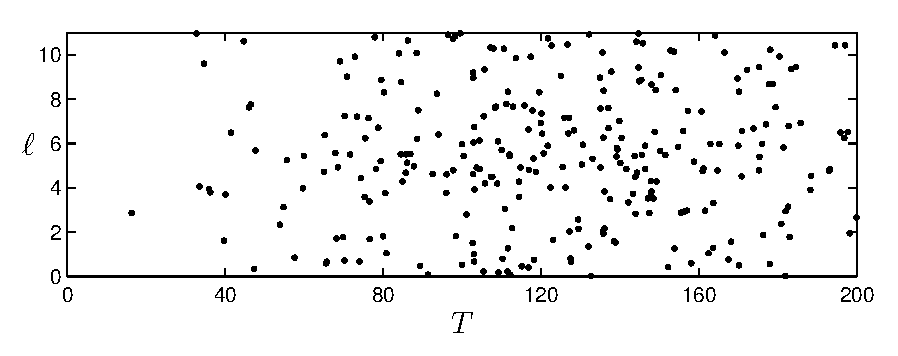
\includegraphics[width=0.7\textwidth]{figs/ks22_rpos_Tdelta.eps}
\end{center}
\caption{\Rpo s of \KSe\ with period $T$ and phase shift $\Delta$.
        } \label{f:ks22rposT}
\end{figure}

The largest Lyapunov exponent of \rpo s is shown in
\reffig{f:ks22rposL}.

\begin{figure}[t]
\begin{center}
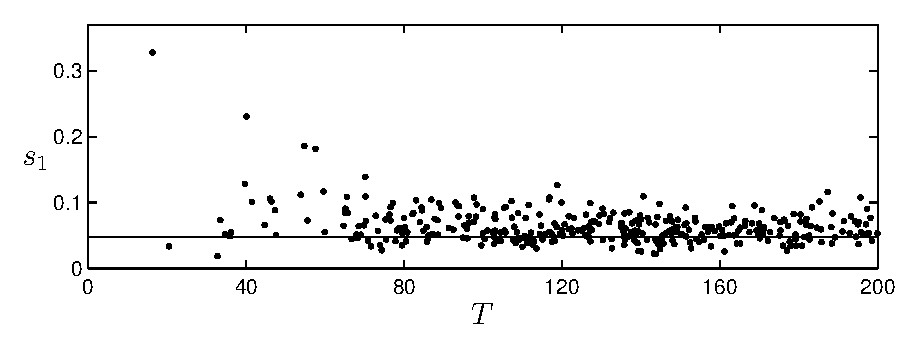
\includegraphics[width=0.7\textwidth]{figs/ks22_rpos_lyap.eps}
\end{center}
\caption{The largest Lyapunov exponent of \rpo s.
        } \label{f:ks22rposL}
\end{figure}

Next we describe several types of \rpo s.

\subsection{Short \rpo s}  The small period \rpo s outline the
coarse structure of the chaotic attractor, while the longer period
\rpo s typically just resolve the finer details of the dynamics
without significant modification of this structure.

The first five orbits with the shortest period we have found are
shown in \reffig{f:ks22rposShort}.  The shortest orbit with $T =
16.4$ is also the most unstable, with one positive Lyapunov exponent
equal 0.328.  The other short orbits are less unstable, with the
largest Lyapunov exponents in the range 0.018 -- 0.073.  The
Lyapunov exponents of a \rpo are given by the formula
\[h_j = \log |\lambda_j|/T\,,\]
where $\lambda_j$ are the eigenvalues of $g(\Delta)J^T(a)$.  The
orbit with $T = 20.5$ is exactly periodic due to a special symmetry
it possesses (see Section~\ref{ssec:po}).

\begin{figure}[t]
\begin{center}
\includegraphics[width=0.9\textwidth]{figs/ks22rposShort.eps}
%(a)\includegraphics[width=0.18\textwidth]{figs/ks22rpo016.3-02.86.eps}
%(b)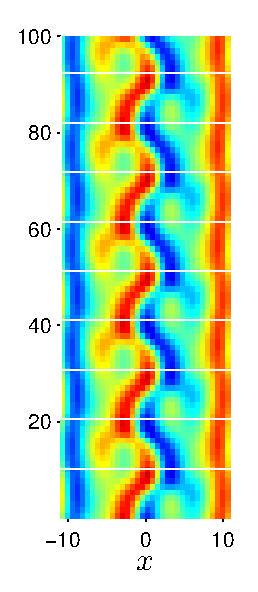
\includegraphics[width=0.18\textwidth]{figs/ks22rpo020.5-00.00.eps}
%(c)\includegraphics[width=0.18\textwidth]{figs/ks22rpo032.8-10.96.eps}
%(d)\includegraphics[width=0.18\textwidth]{figs/ks22rpo033.5-04.04.eps}
%(e)\includegraphics[width=0.18\textwidth]{figs/ks22rpo034.6-09.60.eps}
\end{center}
\caption{Small period \rpo s of \KS equation with $L = 22$: (a) $T =
16.3$, $\Delta = 2.86$; (b) $T = 20.5$, $\Delta = 0.00$ (periodic
orbit); (c) $T = 32.8$, $\Delta = 10.96$; (d) $T = 33.5$, $\Delta =
4.04$; (e) $T = 34.6$, $\Delta = 9.60$.  Horizontal and vertical
white lines indicate periodicity and phase shift of the orbits,
respectively. }\label{f:ks22rposShort}
\end{figure}


\subsection{\Rpo s close to the unstable manifold of \EQV{2} }
We have found a number of \rpo s which stay very close to the
unstable manifold of \EQV{2}.  This confirms that the "cage" of
unstable manifolds of equilibria plays an important role in
organizing the chaotic dynamics of \KS\ equation.

\begin{figure}[t]
\begin{center}
\includegraphics[width=0.9\textwidth]{figs/ks22rposCage.eps}
\end{center}
\caption{\Rpo s close to the unstable manifold of \EQV{2}
equilibrium. (a) $T = 47.6$, $\Delta = 5.68$; (b) $T = 55.6$,
$\Delta = 5.25$; (c) $T = 59.9$, $\Delta = 5.44$; (d) $T = 71.7$,
$\Delta = 5.503$; (e) $T = 85.8$, $\Delta = 5.503$. Horizontal and
vertical white lines indicate periodicity and phase shift of the
orbits, respectively. }\label{f:ks22rposCage}
\end{figure}

\subsection{Periodic Orbits} \label{ssec:po}
A \rpo will be exactly periodic, i.e. $\Delta = 0$, if it has one of
two symmetries: 1) $-u(-x,0) = u(x,0)$ or 2) $-u(-x,T/2) =
u(x,0)$.\RLD{I have the feeling that it can be proven that there are
no other types of symmetries that lead to exactly periodic
solutions, but I don't know how to construct such a proof} In the
first case the whole orbit lives within the antisymmetric subspace.
The dynamics of \KS\ equation in the antisymmetric subspace has been
investigated in [include references]. The \KS\ equation with $L =
22$ does not have any periodic orbits of this type.\RLD{Is it really
so?}

The second symmetry implies that the \rpo\ is reflection-symmetric
to itself after the time translation by half the period.

We have found 21 exactly periodic orbits (POs) with $T < 200$.  The
shortest such orbit is shown in \reffig{f:ks22rposShort}(b).  Some
of the other periodic orbits are shown in \reffig{f:ks22rposPO}. Six
of the 21 POs were found by the same method as used for locating
RPOs, while the other orbits were found by directly employing the
symmetry of the PO:
\[ -u(-x+d,T/2) = u(x,0)\,, \quad -L/2 < d \leq L/2\,.\]
In the Fourier space representation, this symmetry is expressed as
follows
\[
 -{\bf g}(d)a^\ast(T/2) = a(0)\,,
\]
and can be used directly to find a PO with period $T$ (compare it to
the condition (\ref{eq:RPOcond}) for RPOs). \RLD{It looks like there
might be many more POs than I initially expected to find. In fact, I
can even venture a guess that there are approximately as many POs
with symmetry (2) within $T < 200$ as there are RPOs within $T <
100$. The reasoning is that it shouldn't be any harder to match
$-u(-x+d,T/2)$ and $u(x,0)$, than it is to match $u(x+d,T)$ and
$u(x,0)$, provided the dynamics is equally mixing for all types of
orbits.  If this is true, then the number of POs with period smaller
than $T/2$ should be approximately equal to the number of RPOs with
period smaller than $T$; the equality improving with increasing
$T$.}


\begin{figure}[t]
\begin{center}
\includegraphics[width=0.9\textwidth]{figs/ks22rposPO.eps}
\end{center}
\caption{Periodic orbits of \KS\ equation with $L = 22$: (a) $T =
66.8$; (b) $T = 87.2$; (c) $T = 95.3$; (d) $T = 96.4$; (e) $T =
132.6$.}\label{f:ks22rposPO}
\end{figure}


\subsection{Least unstable \rpo s ???}

The dynamics in this small system is competition between wavenumbers
2 and 3. The 2-\eqv\  and the 3-\eqv\  essentially lie in
the 2nd and 3rd Fourier component complex plane, with very
small deformations from higher harmonics.
Hence plot all \rpo s in these 2 representations:

$[ \Re a_2, \Im a_2, \Re a_3 ]$
(here 2-\eqv\  is a circle, 3-\eqv\ a vertical line)
 and
$[ \Re a_3, \Im a_3, \Re a_2 ]$
(here 3-\eqv\ is a circle, 2-\eqv\ a vertical line)

\ES{
The names of the \rpo\ figure files follow the convention
 {\tt rpoL-T-d.eps}s, with suffixes {\tt cm}
and {\tt u} indicating
 mean velocity frame  and $u$ representation respectively.
   }
%
Out of 30 \rpo s we
find,  only three are truly periodic.  The orbit
with $\period{p} = 95.25$ has a very small
$d = -6.5\,\times 10^{-7}$, but it is not periodic
(we
checked this by decreasing the integration step size and increasing the
number of modes).


%%%%%%%%%%%%%%%%%%%%%%%%%%%%%%%%%%%%%%%%%%%%%%%%%%%%%%%%%%%%%%%%
\begin{figure}[t] \label{f:rpo55}
\begin{center}
(a) 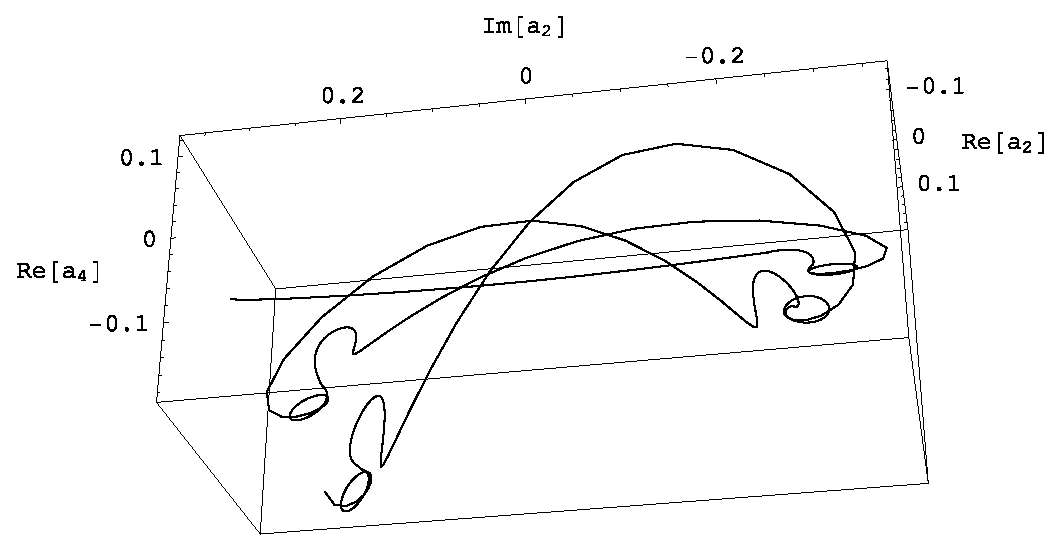
\includegraphics[width=0.35\textwidth]{figs/rpo22-55-4-clean.eps}
% ./removecache.sh rpo22-55-4.eps
% abandoned rpoEq22-55-4.eps with mean velocity equilibrium embeded.
(b) 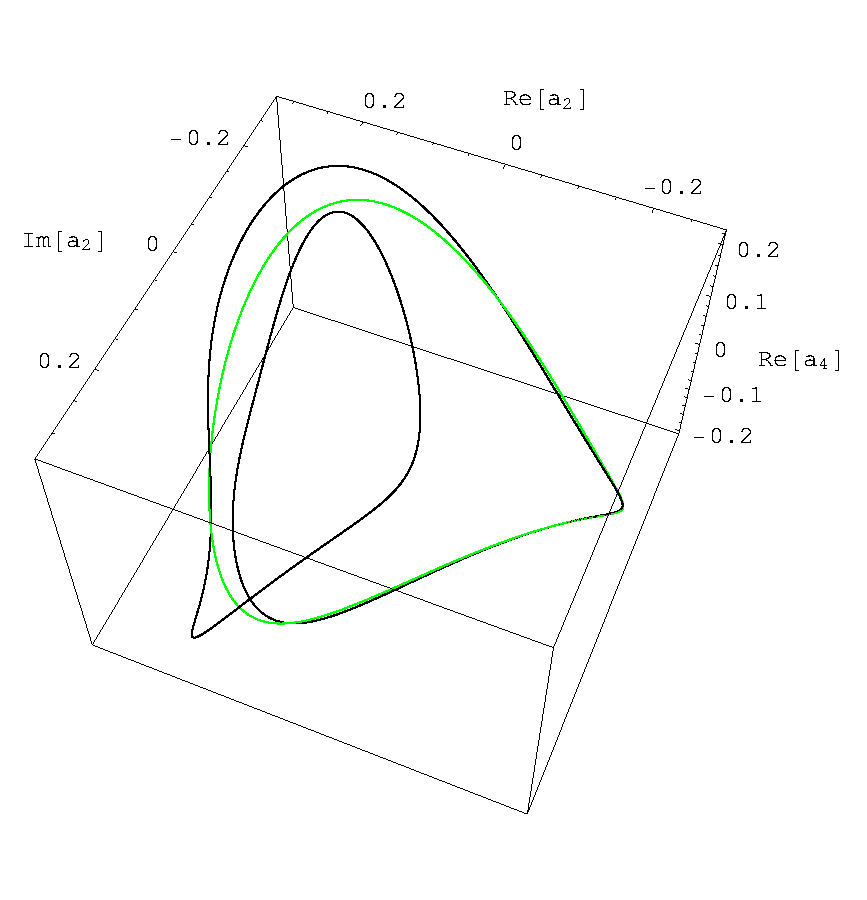
\includegraphics[width=0.25\textwidth]{figs/rpoEq22-55-4-cm.eps}
(c) [create rpoEq22-55-4-cm-?.eps]
\end{center}
\caption{
 The \rpo\ {\nameit}55 in:
 (a) \Statesp, traced for four periods $\period{p}$.
% Green curve belongs to \reffig{f:rpo55}(b) % rpo22-55-4-cm.eps
% rather than to  \reffig{f:rpo55}(a), % rpoEq22-55-4.eps?
 (b) mean velocity frame.
        The continuos family of
    {\eqva} A obtained by the action of $g$ is shown in green,
    the SA family shown in red. The \rpo\ {\nameit}55 stays close
    to either A or SA for close to 1/2 of {\eqv} rotation
    period, then quickly jumps to the other {\eqv} point.
 (c) mean velocity frame A, SA and {\nameit}55 projected on the
    $[a_?,a_?]$ plane,
    with the $\sigma x = -x$ symmetry of \KSe\ explicit.
        }
\end{figure}
%%%%%%%%%%%%%%%%%%%%%%%%%%%%%%%%%%%%%%%%%%%%%%%%%%%%%%%%%%%%%%%%%%



Sets of \rpo s are difficult to visualize simultaneously.
For ordinary \po s one
plots the unstable plane of the \eqv, shows where the periodic
orbits sit. Other options:

Somewhat better visualization is in the
{\em mean velocity frame}, {\ie}
a reference frame that rotates with with velocity
$v_p=d_p/\period{p}$
In the mean velocity frame a \rpo\ becomes
a \po, see  for example \refeq{f:rpo55}.
Mean velocity frame visualization helps quite a bit.
Put a black (green, respectively) dot
twice thickness of the line every time unit; it will enable you to see
where the motion is slow and where it is fast.
% (a trick we used to understand plane Couette trajectories).
Mark the initial point on both
mean velocity \rpo\ and on \eqv\  in mean velocity
 frame with a fat triangle
indicating the direction, so we can see how they both move. Probably at the
opposite ends of the two curves - mean velocity frame is the mean motion.

%   rpo/figs/detail1rpo22-55-4.eps
%   rpo/figs/detail2rpo22-55-4.eps
%   rpo/figs/detail3rpo22-55-4.eps
%   break rpo22-55-4 into 3 parts.
%   The script for the fonts somehow crops these images

Each {\rpo} has its own mean velocity frame - and within it, {\eqv}
move on circles (or worse - because in higher Fourier modes they do more
complicated things), and it is important to know where the {\eqv} is at
a given instant.

As the shift $d$ is defined mod~$L$, better to
state for each {\rpo} its mean velocity $c_p = d_p/\period{p}$,
where $d_p$ is measured on the line (not on the circle). $c_p$ is
preferable to angle $2\pi d_p/L$ as it does not vary in $L \to$~large
limit (just like $\sqrt{2}$ wavelength estimate is independent of
system size.

Another convenient way to plot \eqva\ and \reqva\ on a periodic
domain $L$ is to plot
$\partial u(x)$ vs. $u(x)$ as a curve parametrized by
$x\in [0,L]$. In this representation both \eqva\ and \reqva\ curves are
stationary, but the points on \reqva\ move as functions of time.

\Po s and \rpo s can be plotted this way as well
$\partial u(x,t)$ vs. $u(x,t)$. Now they are are represented by time-dependent
``tube".

\refFig{f:ks22RE}(b)
depicts \REQV{+}{2}.
It belongs to the branch starting at point $M$
\PC{does it start at M?}
in bifurcation diagram \reffig{fig:ksBifDiag}.
It has one real unstable eigenvalue = 0.337,
so it is more unstable than \REQV{+}{1},
but only in 1\dmn\ (\REQV{+}{1} is unstable in 4\dmn).
\PC{removed Ruslan Feb 8 2007 Fig f:TW1TW2.ps in favor of fresher version}
